\documentclass[10pt]{article}
%\documentclass[10pt]{tufte-handout}


\usepackage[utf8]{inputenc}
\renewcommand*{\familydefault}{\sfdefault}

\usepackage{graphicx}      
\usepackage{hyperref}       
\usepackage{amsmath, amssymb}

\usepackage{fullpage}


\usepackage{subfigure}
\usepackage{tikz}


\parindent0pt
\parskip5pt

\title{A probabilistic model for information need in information retrieval}
\author{A1, A2}
\date{}

\begin{document}
\maketitle
\begin{abstract}
 A probabilistic model for information need in information retrieval is derived from the basic problem definition. The model is shown to work on various example scenarios, and extensions such as new modes of feedback are discussed.
\end{abstract}

\section{Introduction}
{\it Information retrieval is the activity of obtaining information resources relevant to an information need from a collection of information resources.} -WP

{\it Information retrieval (IR) is finding material (usually documents) of an unstructured nature (usually text) that satisfies an information need from within large collections (usually stored on computers).} - http://nlp.stanford.edu/IR-book/html/htmledition/irbook.html

What IR is not in this paper: recommender systems, 'proactive' (=recommender systems), browsing, filtering.

The continuum from exact item match to exploration of new consepts. Where to draw the line between IR and browsing.



\section{Definition}

Definitions in literature, common denominator at a conceptual level.

\subsection{Problem}
An information retrieval system needs to solve the problem of incomplete knowledge of user's information need. Key components must be defined in order to realize any such system.

First component is a known collection $C$ of retrieval items. Each item $i \in C$ in the collection must have a quantification: Call such quantification the feature representation $x_i\in \mathcal X$ in some suitable space $\mathcal X$. For example, a piece of music can be described by the artist, title and record labels, each represented as value 1 of a corresponding binary variable in the joint space of all possible artist, title and record names, together with other features such as length, bitrate, spectral moments etc.

Second component is the representation of information need. This can be formalized by equating the information need $\theta$ with a distribution in the feature space. For example, with some parametric distribution family $p_\theta$ we would set $P(event\ A) = \int_A p_\theta (x) dx$.

Third component is the representation of item relevance, expressed as a scalar variable $r_i\in \mathbb R$. A typical choice interprets low value as 'not relevant' and high value as 'relevant'. The unit interval is common, and even the binary model is often used, with the downside of e.g. losing 0.5 as 'irrelevant'.

Assume also that the collection is too big or that items are too complicated to simply visualize the entire collection.

\subsection{Solution}
The three components $ \theta, x_i, r_i$ are now connected to make the dependency graph of a solution. Note that the minimal solution graph has at least two edges, as any less would render a component independent of the other two and our problem definition redundant.

\begin{figure}%
\subfigure[All possible interactions between the variables.]{
\begin{tikzpicture}[node distance=8em]
  \node[] (doc) {$x_i$};
  \node[above right of=doc] (rel) {$r_i$};
  \node[above left of=doc] (theta) {$\theta$};

  \draw[] (theta) -- node [left] {1.} (doc);
  \draw[] (doc) -- node [right] {2.} (rel);
  \draw[] (theta) -- node [above] {3.} (rel);
\end{tikzpicture}
}
\subfigure[Pruned interactions]{
\begin{tikzpicture}[node distance=8em]
  \node[] (doc) {$x_i$};
  \node[above right of=doc] (rel) {$r_i$};
  \node[above left of=doc] (theta) {$\theta$};

  \draw[] (doc) -- (rel);
  \draw[] (theta) -- (rel);
\end{tikzpicture}
}
%\subfigure[Possible effect directions between information need and
%  relevance.]{
%\begin{tikzpicture}[node distance=5em]
%  \node (theta) {$\theta$};
%  \node[right of=theta] (rel) {$r_i$};
%  
%  \draw[->] (theta) -- (rel);
%\end{tikzpicture}
%
%\begin{tikzpicture}[node distance=5em]
%  \node (theta) {$\theta$};
%  \node[right of=theta] (rel) {$r_i$};
%  
%  \draw[<-] (theta) -- (rel);
%\end{tikzpicture}
%}
%\begin{tikzpicture}[node distance=5em]
%  \node (doc) {$x_i$};
%  \node[right of=theta] (rel) {$r_i$};
%  
%  \draw[->] (doc) -- (rel);
%\end{tikzpicture}
\subfigure[Solution.]{
\begin{tikzpicture}[node distance=8em]
 \node[] (doc) {$x_i$};
  \node[above right of=doc] (rel) {$r_i$};
  \node[above left of=doc] (theta) {$\theta$};

  \draw[->] (doc) -- (rel);
  \draw[->] (theta) -- (rel);
\end{tikzpicture}
}
\caption{Derivation of the solution graph.}
\label{fig:graph1}
\end{figure}

The complete graph (Figure~\ref{fig:graph1}a) is not useful: consider
the two possible cases of interaction between $\theta$ and $x_i$. If the user's information need would
affect the feature representation, the change of a user would violate
the first assumption of a fixed collection. Vice versa, the feature
representation should not affect what the user is looking for, but
affect only the system's internal operation. 

The solution has two edges, connecting the information need with the items through
relevance (Figure~\ref{fig:graph1}b). The next step is to argue effect direction. Consider the interaction between $\theta$ and $r_i$. Natural direction of effect is that infromation need defines what is the relevance of an item. The other direction would imply that the items have some user independent state of relevance, and hence the system would not be providing the user relevant item, but penalize users with non-relevant needs (T: not good... need more thought).

Similarly for $x_i$ and $r_i$: if the items are modeled using their relevances then each item would have a different representation when relevances change. The final solution models the relevance variable as a function of information need and fixed item features (Figure~\ref{fig:graph1}c). In probabilistic form the model is written as $p(r_i|\theta, x_i)$. 
\subsection{Data collection}
In order to estimate the information need $\theta$ some data collection mechanisms are required. For example, a textual query can be entered by the user. Another direct approach is to ask the user some values of $r_i$ on some visualized set of items $i$. In general we presume that data provided by the user is dependent on the information need. Following arguments by   Lavrenko 2004 we presume that all data given by the user is an impresize and constrained stochastic expression of $\theta$, i.e. any use action mechanism $a_\star$ is modelled as $a_\star \sim p(\cdot| \theta)$ (Figure~\ref{fig:graph2}). The form of the user action models depend on the system realisation.

\begin{figure}[!h]
\centering
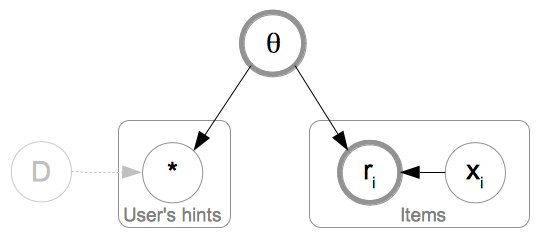
\includegraphics[scale=.35]{figures/user-model.png}
\caption{Graphical model describing the interactions between information need, item relevance and user actions (or hints).}
\label{fig:graph2}
\end{figure}



%Other sources of data include feature-wise relevance feedback, ordering (preference) feedback, 

%Pseudo-feedback

\subsection{Example systems}
First example system has the linear item relevance model with coefficients given by the information need, i.e.
\begin{eqnarray}
r_i | x_i, \theta & \sim & N(\theta^T x_i, \sigma^2)
\end{eqnarray}
As often it suffices to know the relative values of $r_i$, e.g. for presenting ranked lists of results, the $\sigma_2$ parameter can be set to any value or the model can be replaced by the linear function $r_i = \theta^T x_i$. 

Let's assume the user provides an input $y$, e.g. textual query. Several options for connecting the input to the information need now emerge. The naive approach is to relate the input to a relevant item by mapping it to the feature space $y \mapsto x_{y}$, and interpreting $r_y$ and $x_y$ with some high value of $r_y$ as a sample from the item relevance model. The OLS solution $\hat \theta = (x_y x_y^T)^{-1}x_y r_y$ is then used for predicting $r_i$ for the documents. The problem is overparameterised but we omit such details for now. 

If we omit the model details and jump from query to relevances and apply a crude diagonalization approximation of the inverse gives, the system's task is to compute
\begin{eqnarray}
r_i/r &=& \sum_k^P x_{yk} x_{ik}\\
\end{eqnarray} 
This relates to the popular cosine similarity approach when the vectors are of unit length. The unit length assumption can be inplemented to the statistical model via either suitable choise of $r_i$ values or by tuning $\sigma^2$. 

Second item relevance model is the logistic model
\begin{eqnarray}
r_i | x_i, \theta & \sim & Bernoulli(\pi_i)\\
\log \frac{\pi_i}{1-\pi_i} &=& \theta^T x_i
\end{eqnarray}
If the input model now uses the item relevancy model, $r_y=1$ is chosen. More realistic input model is one that accounts for the visualization. Let the system have a ranked list visualization, and assume that the user's input for each item in the list depends inversely on the list position $s_i=1,...$.  To model inputting on each item $i$, define an auxiliary variable $z_i$ for observing relevance feedback on item $i$. The relevance of item $i$ is observed if $z_i=1$, and missing if $z_i=0$. The connection between information need and the input is then given by 
\begin{eqnarray}
y & \sim & p(r_y=1 | x_y, \theta) p(z_y=1 | s_y, \theta')
\end{eqnarray}
where $\theta'$ was used for generating the visualization (e.g. the previous iteration estimate).  

\section{Properties}

In this section we have interpretation of higher level quantities. Session, information drift, precision-recall, feedback.

\subsection{Definitions of consepts in IR systems}
A session is a bounded and continuous period of system use. Assumption of a constant information need $\theta$ over a session implies constant item relevances and the IR problem is solved by statistical estimation using all data gathered during the session. The problem of session boundary detection is solved by change-point detection in the value of $\theta$. 

Alternative to a fixed $\theta$ is a drifting or shifting information need, reflecting the user's learning or remembering over time. To define a session in such a case requires an extra variable $\Theta$ to represent the larger task involving the information retrieval task. Then $(\theta_t)_{t=1}^T$ is an (autocorrelated) realisation of $\Theta$ over time, i.e. a process approach is needed.

The information need is not possible to be observed in full as this would negate the need for probabilistic retrieval ('retrieve exactly this' is redundant). Querying, item rating and other data collection mechanisms built to the user interface are inprecise and constrained ways for user to give the system some hints of the information need $\theta$. Each mechanism is to be modelled individually as a variable dependent on the information need. For example, query strings and relevance feedback clicks on ranked items are both stochastic expressions originating from the same underlying $\theta$, but their execution mechanisms and informativeness are different.

Extra sources of data are often used to minimize the user's burden of providing hints. The user's previous sessions can be used as additional data, with some weighting scheme to account for information need jumps and shifts between sessions. Profiles can be build using some classification rules on user's previous session data. The idea is to build a set of hypothetical states $\theta^1, ..., \theta^m$ which the user is assumed to exhibit, and as the information need space is reduced, the IR problem is reduced to mixture distribution weight estimation.

Another technique is to borrow data from other users. The system is build on some tuneable balance between the population and the individual's information needs. The population homogeneity assumption holds in some applications, e.g. it is often valid to presume that "each user wants high pagerank web search results", but $\theta$ values can be, partially or fully, more heterogeneous for any given set of hints when the users' tasks vary considerably. Historically the IR problem have been solved using population averages. Personalization becomes available through detailed user modeling and informative system interfaces.

Evaluation of the retrieval: precision-recall, diversity, etc.

The conditional nature of the solution: User's information need given the feature space and collection. Does it match the problem.

\subsection{Latent variable models and Bayesian inference}

The Bayesian approach, the idea of prior knowledge and how profiling etc. are naturally covered.

Borrowing data and the informativeness of a prior.

(T: should the previous subsection descriptions of consepts be here, so the Baysian way could be easily incorporated? Would avoid repetition.)
\subsection{Comparison to previous definitions of probabilistic IR}



\section{Examples}

\section{Discussion}


\end{document}  
